\chapter{Analysis Techniques}
\label{app:AnalTech}
\chapterquote{think of a quote}%
{quote}

Thus far in this thesis, we have covered the theory of particle physics, how we detect and reconstruct the particles and the MC techniques. Yet a some questions still remain, such as: How do we separate events the into a signal and background event? And how do we construct a statistically robust framework, using our signal and background events? To answer the first question, usually a multivariate analysis incorporating a machine learning technique is used. For the $t\bar{t}H(b\bar{b})$ analysis a  multi-class neural network based on a permutation-invariant transformer architecture with attention mechanism is used \cite{attentionisallyouneed}. Using the output of this framework a combined profile likelihood fit that simultaneously determines the event yields for the signal and for the most important background components, while constraining the overall background model within the assigned systematic uncertainties is constructed.\\
\\
This chapter will serve as a general introduction to the transformer architecture and profile likelihood fit construction before we apply these concepts in Chapter \ref{chap::tth}.

\section{Profile Likelihoods}
\subsection{Poisson Distributions}
In each $pp$ collision at the LHC, the final state may originate from the signal process or from a variety of background processes. These cannot be separated event-by-event with perfect accuracy, but their relative contributions can be inferred statistically using the measured distributions in signal- and control-enriched regions. The data in these regions are organized into histograms of discriminant variables, such as the output of a neural network classifier or a reconstructed mass or Higgs $p_T$. Each of these events has a small probability of producing the final state of interest. This matches the conditions under which the Poisson distribution applies: rare independent trials with a constant rate. The Poisson model correctly describes both low-statistics bins and high-statistics bins (where it smoothly approximates a Gaussian). Therefore, the likelihood in each bin is taken as the Poisson probability of the observed count given the predicted mean from signal and background. We define the Poisson distribution as:
\begin{equation}
P(n |\nu) = \frac{\nu^n e^{-\nu}}{n!},
\end{equation}
where $\nu$ is the expected mean yield in the bin, determined from the signal and background model.  $n$ is the observed number of events in the bin. $e^{-\nu}$ ensures that the total probability over all $n \in \{0,1,2,\dots\}$ sums to one. The factorial $n!$ accounts for the number of distinct permutations of $n$ indistinguishable events.
\subsection{The Likelihood Function}
The likelihood function, denoted $\mathcal{L}(\boldsymbol{\Theta})$, quantifies the probability of observing the data $x$ given a set of model parameters $\boldsymbol{\Theta}$. In other words, it measures the degree to which a model, parametrised by $\boldsymbol{\Theta}$, agrees with the observed data. For a set of $n$ statistically independent measurements $x_1, x_2, \dots, x_n$, each described by a probability density function $f(x;\boldsymbol{\Theta})$, the likelihood is given by:
\begin{equation}
\mathcal{L}(\boldsymbol{\Theta}) = \prod_{i=1}^n f(x_i \;|\; \boldsymbol{\Theta}).
\end{equation}
The assumption of independence allows the likelihood to factorise as a product of the individual PDFs, such that:
\begin{equation}
    P(x_1, x_2, \dots, x_n | \Theta) 
= \prod_{i=1}^n P(x_i | \Theta).
\end{equation}
In practice, it is more convenient to work with the logarithm of the likelihood. Taking the logarithm converts the product into a sum:
\begin{equation}
\ln \mathcal{L}(\boldsymbol{\Theta}) = \sum_{i=1}^n \ln f(x_i | \boldsymbol{\Theta}).
\end{equation}
It is standard in high-energy physics to minimise the negative log-likelihood:
\begin{equation}
-\ln \mathcal{L}(\boldsymbol{\Theta}) = - \sum_{i=1}^n \ln f(x_i| \boldsymbol{\Theta}),
\end{equation}
since optimisation algorithms are typically designed to locate minima of functions. Minimising the negative log-likelihood is mathematically equivalent to maximising the likelihood\footnote{Its always easier to differentiate a sum than a product.}.
\subsection{The Likelihood Function With Binned Data}
For the $t\bar{t}H(b\bar{b})$ legacy analysis in Chapter \ref{chap::tth} the model parameters are: signal strength $\mu$, normalisation factors $k$ and the set of Nuisance Parameters (NPs) $\theta$ (these are usually modelled as Gaussian priors), which we use to describe the effects of systematic uncertainties in the expectations and treated as extra degrees of freedom inside the fit. For a binned distribution, the number of expected events for bin $i$ can be expressed using the experimentally observed number of events in bin $i$, given by:
\begin{equation}
    N_i^{\text{exp}}(\mu,k,\theta)= \sum_s \mu_s \cdot N_{\text{Sig},i}^s (\theta) + \sum_b k_b \cdot N_{\text{Bkg},i}^b (\theta), 
\end{equation}
where $N_{\text{Sig},i}^s$ is the number of expected signal events from a signal process $s$ in bin $i$. $N_{\text{Bkg},i}^b$ is the number of background events for a given background process $b$ in bin $i$. $\mu_s$ and $k_b$ are the signal strength and background normalisation factor for a given background process. These background normalisation factor(s) can either be set to one, assuming exactly SM like behaviour or left to freely float with an initial value of one, allowing the fit to then adapt to observed and expected number of events. The signal strength is given by:
\begin{equation}
    \label{mu}
    \mu_s = \frac{\sigma^s}{\sigma_{\text{SM}}^s},
\end{equation}
where $\sigma^s$ is the observed cross-section of the measured signal process, $s$ and $\sigma_{\text{SM}}^s$ is the expected SM cross-section for the same process. When quoting signal strength for an inclusive measurement only one $\mu$ is used. For a Simplified Template Cross-Section\footnote{This is aa agreed framework that partitions Higgs production processes into kinematic regions to enable precise, model-independent measurements of Higgs properties.} (STXS) measurement a $\mu$ is used for each STXS region.The resulting binned likelihood function is given my:
\begin{equation}\label{binnedlikelihood}
    \mathcal{L}(\mu,k,\theta) = \prod_i^M\frac{N^{\mathrm{exp}}_i(\mu, k, \theta)^{N_i}}{N_i!} \; e^{-N^{\mathrm{exp}}_i(\mu, k, \theta)},
\end{equation}
where $M$ is the total number of bins and $N_i$ is the number of events in bin $i$. Equation \ref{mu} shows that large or small values of cross-section can lead to speculation of the presence of new physics, provided no large systematic or modelling uncertainty dominates this potential deviation. A change of bias ($\mu \rightarrow$Wilson Coefficient) in Equation \ref{binnedlikelihood} can be used to re-interpret a SM measurement in the EFT framework discussed in Section \ref{sec:SMEFT}.
\subsection{Profile Likelihoods and Test Statistic}
The profile likelihood fit is the statistical framework used to extract the best-fit value of a Parameter Of Interest (POI). Here its $\mu$, while consistently incorporating the effects of systematic uncertainties Nuisance Parameters (NPs) and normalisation factors. In this approach, for each tested value of $\mu$, the likelihood is maximized with respect to all nuisance parameters, yielding the profile likelihood:
\begin{equation}
    \mathcal{L}(\mu) = \mathcal{L}(\mu,\hat{\hat{k}}, \hat{\hat{\theta}}),
\end{equation} 
where $\hat{\hat{\theta}}$ is the value of a given NP that maximizes the likelihood for a fixed value of $\mu$. The value of $\mu$ that maximizes the full likelihood function is the best-fit signal strength $\hat{\mu}$, and the shape of the profile likelihood around $\hat{\mu}$ determines the statistical uncertainty. The ratio of these two likelihood methods is given by $\lambda_\mu$:\begin{equation}
    \lambda_\mu = \frac{\mathcal{L}(\mu,\hat{\hat{k}}, \hat{\hat{\theta}})}{\mathcal{L}(\hat{\mu},{\hat{k}}, {\hat{\theta}})}
\end{equation} 
To quantify the compatibility of different $\mu$ values with the observed data, the test statistic is defined as:\begin{equation}
    q_{\mu} = -2 \ln \lambda_\mu
\end{equation}
This test statistic is used both to construct confidence intervals for $\mu$, and to quantify the level of compatibility between the observed data and the hypothesis parameter setting $\mu$. Larger values of $q_\mu$ correspond to observed data is less compatible with the hypothesised value of $\mu$.
\subsection{Significance}
The deviation from the background-only hypothesis is quantified by the signal significance $S$, defined as:  
\begin{equation}
S = \sqrt{\lambda_0},
\end{equation}
where $\lambda_0$ is the likelihood ratio evaluated at $\mu=0$ (background only). The significance expresses how strongly the observed result deviates from the background-only expectation, typically quoted in units of standard deviations ($\sigma$). In particle physics, two common thresholds are used: a significance of at least $3\sigma$ is referred to as evidence, corresponding to a $p$-value of approximately $0.3\%$, while a significance of $5\sigma$ is required for a discovery, corresponding to a $p$-value of about $3\times10^{-7}$. Here, the $p$-value represents the probability of observing a deviation as large as, or larger than, the measured result under the assumption that the background-only hypothesis is true.

\subsection{Nuisance Parameter Pulls}
NPs nominally have a central value of $\theta = 0$, describing the best possible value associated with a given systematic uncertainty. If this central value were to shift we call this a pull in our fit, which is described as: 
\begin{equation}
    \text{Pull} = \frac{\hat{\theta} - \theta_0}{\Delta\theta},
\end{equation} 
where $\hat{\theta}$ is the fitted value of the NP, $\theta_0$ is the nominal (pre-fit) value and $\Delta\theta$ is the uncertainty of that NP (pre-fit or post-fit, depending on convention). These pulls can indicate potentially problematic modeling parameters or tensions in the fit. As a diagnostic tool a significant pull is usually the first step in any statistical detective work when trying to understand problems in the fit. 
\subsection{Asimov Data Sets}
An Asimov fit is performed using a specially constructed dataset where each bin contains exactly the expected yield from the model without any statistical fluctuations. This dataset represents the median expectation under a given hypothesis (often the SM signal strength
$\mu=1$ or the background-only case $\mu = 0$). Fitting the Asimov dataset allows one to evaluate the expected performance of the analysis, such as the anticipated uncertainty on the signal strength, the ranking of nuisance parameters, and the pulls on NPs, in the absence of statistical noise. By comparing the results of an Asimov fit to the fit on real data, one can identify deviations in nuisance parameter pulls or impacts that may indicate tensions between data and the model or underestimated systematic uncertainties. These comparisons are another key tool in the statistical detective's repertoire. 
\subsection{Tools Used}
To use the statistical framework we have described thus far a number of tools are used. Namely tools provided by the RooStat framework \cite{roostats1,roostats2}, which is applied using the TRExFitter framework, and is based on the HistFactory framework \cite{histlab}. The minimisation is performed using the Minuit library implemented in ROOT \cite{minut,root}.




\section{Transformer Neural Networks}
HEP experiments produce vast and complex datasets describing the properties and interactions of subatomic particles. Extracting meaningful patterns from these data has long been a central challenge, historically addressed using carefully engineered features and domain-specific algorithms. In recent years, advances in machine learning (ML) have transformed the analysis landscape, enabling models to learn directly from raw detector outputs and simulation data. Techniques such as boosted decision trees, convolutional neural networks (CNNs), and graph neural networks (GNNs) have all demonstrated remarkable performance in classification, reconstruction, and anomaly detection tasks.\\
\\
Transformers represent the next stage in this evolution. Originally developed for natural language processing, transformers replace sequential recurrence with a global attention mechanism, allowing the model to capture long-range and complex dependencies between input elements. This architecture is highly flexible: by treating the input as a set of feature vectors rather than an ordered sequence, transformers can naturally operate in a permutation-invariant fashion.\\
\\
In this Section, we present the core components of the transformer architecture, with emphasis on the attention mechanism and its adaptation to HEP data. We describe how input particle features are embedded, how self and cross-attention layers propagate information, and how the overall architecture can be constructed to preserve physical symmetries. The goal is to illustrate why transformers are a powerful and for the classification and reconstruction problems faced by the $t\bar{t}H(b\bar{b})$ Analysis. All components of this discussion are taken from \cite{UDL}.
\subsection{The Attention Mechanism}
The Transformer architecture uses attention mechanisms to capture connection between the input representations\footnote{input representations are just input features, which is our raw data, post embedding.}. These connections are derived via dot-product self attention which transforms the input data in to Queries, Keys and Values, with attention weights to computed according to the feature in question. The final architecture for the transformer is represented by a stack of shallow networks with blocks of self attention to allow for the exchange of relevant information, giving rise to a more expressive model compare to traditional neural networks. Let us begin to build the concepts for this architecture and start with dot-product self attention.
\subsubsection{Dot-Product Self-Attention}
The core operation of self-attention, denoted \textbf{sa[$\bullet$]}, is to determine the relevance of one input object to another via a similarity measure. 
Given a set of $N$ input vectors 
$\{x_1, x_2, \dots, x_N\}$, where $x_m \in \mathbb{R}^{D \times 1}$\footnote{In the context of the $t\bar{t}H(b\bar{b})$ analysis the inputs will be particle objects such as $p_T$, mass, PCBT bin and so on.},
we first compute a \emph{query} vector $q_n$ for the object and a \emph{key} vector $k_m$ for each object in the set:
\begin{equation}
q_n = b_q + \Omega_q x_n, \quad k_m = b_k + \Omega_k x_m,
\end{equation}
where $\Omega_q, \Omega_k \in \mathbb{R}^{D \times D}$ are learnable weight matrices and $b_q, b_k \in \mathbb{R}^D$ are biases. The layman’s understanding of the query is simply ``what this input object is looking for'' in the other input objects. 
Similarly, a key can be thought of as ``what an input object has to offer'' for comparison, while the value is the actual information that will be shared if that object is deemed relevant. The similarity between the query of one object and the key of another is computed using the scaled dot product between $q_n$ and $k_m$:  
\begin{equation}
s_{nm} = \frac{q_n^\top k_m}{\sqrt{d_k}},
\end{equation}
where $d_k$ is the dimensionality of the keys. The scaling factor $1/\sqrt{d_k}$ prevents the dot products from becoming large in magnitude, which would otherwise push the softmax into regions with small gradients These similarity scores form the basis for computing attention weights, which determine how strongly each input object incorporates information from all others.

\subsubsection{Computing the Attention Weights}

The raw similarity scores $s_{nm}$ quantify how closely the query vector of object $n$ matches the key vector of object $m$. However, these scores are unbounded real numbers and cannot be used directly to weight the values. To convert them into a set of interpretable, non-negative coefficients that sum to one, we apply the softmax function across the $m$ index for each fixed $n$:
\begin{equation}
a[x_m, x_n] = \frac{\exp(s_{nm})}{\sum_{j=1}^N \exp(s_{nj})}.
\end{equation}
The softmax has two important effects: It exponentiates the scores, which accentuates differences between high and low similarity values, thereby sharpening the focus of the attention mechanism. It also normalises the set of scores for each $n$ so that they form a valid probability distribution over the $N$ input objects. These weights satisfy:
\begin{equation}
a[x_m, x_n] \ge 0, \quad \sum_{m=1}^N a[x_m, x_n] = 1,
\end{equation}
meaning they can be interpreted as the fraction of ``attention'' that the updated representation of object $n$ assigns to the information coming from object $m$. 
A large value of $a[x_m, x_n]$ indicates that the features of $m$ are highly relevant to updating $n$, whereas a small value indicates limited influence. 
In the context of the $t\bar{t}H(b\bar{b})$ analysis, these weights encode learned, event-specific relationships between different reconstructed objects, enabling the network to dynamically decide which inputs are most informative for the task at hand.
\subsubsection{From Dot-Product Attention to the Self-Attention Block}
In addition to the queries and keys, each input object $x_m$ is also projected into a value vector:
\begin{equation}
v_m = b_v + \Omega_v x_m,
\end{equation}
where $\Omega_v \in \mathbb{R}^{D \times D}$ and $b_v \in \mathbb{R}^D$ are learnable parameters. This transformation is analogous to the affine mapping in a standard feed-forward layer, but here no non-linear activation is applied. 
The values represent the raw information content associated with each input object that will be shared with others once the attention weights have been determined.The output representation for object $n$ is then computed as a weighted sum over the value vectors of all $N$ input objects:
\begin{equation}
\mathrm{sa}_n[x_1, \dots, x_N] = \sum_{m=1}^N a[x_m, x_n] \, v_m.
\end{equation}
Here, $a[x_m, x_n]$ controls how much of $v_m$ is incorporated into the updated representation of $x_n$. A high attention weight means that the information from object $m$ is strongly relevant to updating $n$, while a low weight means it contributes very little. 
In this way, the self-attention block enables each object to gather contextual information from every other object in the set, producing context-aware representations that are dynamically tailored to the specific event being processed.\\
\\
Because the computation relies only on pairwise similarities between objects and not on their position in the input list, the self-attention operation is inherently permutation-invariant. This property is particularly advantageous in domains, such as the $t\bar{t}H(b\bar{b})$ analysis, where the ordering of reconstructed objects carries no physical meaning.
\subsubsection{Multi-Headed Attention}
\subsection{Multi-Headed Attention and Matrix Formulation}
Up to this point, the description of self-attention has been expressed in terms of individual input objects and their corresponding query, key, and value \emph{vectors}. 
While this view is useful for building intuition, in practice the computation is implemented more efficiently using a \emph{matrix} representation. 
Instead of processing each input $x_m$ separately, all $N$ input representations are arranged into a single matrix:
\begin{equation}
X = 
\begin{bmatrix}
x_1^\top \\
x_2^\top \\
\vdots \\
x_N^\top
\end{bmatrix}
\in \mathbb{R}^{N \times D}.
\end{equation}
The queries, keys, and values for all inputs are then computed in parallel by multiplying $X$ with learned weight matrices and adding a basis matrix:
\begin{equation}
\mathbf{Q} = \mathbf{X} \, \mathbf{\Omega}_Q + \mathbf{1} \, \mathbf{b}_Q^\top, \quad
\mathbf{K} = \mathbf{X} \, \mathbf{\Omega}_K + \mathbf{1} \, \mathbf{b}_K^\top, \quad
\mathbf{V} = \mathbf{X} \, \mathbf{\Omega}_V + \mathbf{1} \, \mathbf{b}_V^\top,
\end{equation}
where $W_Q, W_K, W_V \in \mathbb{R}^{D \times d_k}$ are learnable parameter matrices. 
Here, $\mathbf{Q}$, $\mathbf{K}$, and $\mathbf{V}$ have shapes $\mathbb{R}^{N \times d_k}$, and each row corresponds to the query, key, or value of one input object. The attention mechanism in matrix form can then be written as:
\begin{equation}
\mathrm{Attention}(\mathbf{Q}, \mathbf{K}, \mathbf{V}) = \mathrm{softmax} \left( \frac{\mathbf{Q} \, \mathbf{K}^\top}{\sqrt{d_k}} \right) \mathbf{V},
\end{equation}
where the matrix $\mathbf{Q} \, \mathbf{K}^\top \in \mathbb{R}^{N \times N}$ contains all pairwise similarity scores between queries and keys, the softmax is applied row-wise, and the resulting attention weight matrix multiplies $\mathbf{V}$ to produce the updated representations.

\subsubsection{Multi-Headed Attention}

A single attention head uses one set of parameters $(\mathbf{\Omega}_Q, \mathbf{\Omega}_K, \mathbf{\Omega}_V, \mathbf{b}_Q, \mathbf{b}_K, \mathbf{b}_V)$, which limits it to learning one type of relationship at a time. \emph{Multi-headed attention} overcomes this by introducing $H$ parallel attention heads, each with its own parameters:
\begin{equation}
Q^{(h)} = X W_Q^{(h)}, \quad
K^{(h)} = X W_K^{(h)}, \quad
V^{(h)} = X W_V^{(h)}, \quad h = 1, \dots, H.
\end{equation}
Each head computes its own attention output:
\begin{equation}
\mathrm{head}_h = \mathrm{Attention}\left( \mathbf{Q}^{(h)}, \mathbf{K}^{(h)}, \mathbf{V}^{(h)} \right).
\end{equation}
These outputs are concatenated along the feature dimension and projected back to the model dimension $D$:
\begin{equation}
\mathrm{MultiHead}(\mathbf{X}) = \mathrm{Concat}\left(\mathrm{head}_1, \dots, \mathrm{head}_H\right) \, \mathbf{W}_O,
\end{equation}
where $\mathbf{W}_O \in \mathbb{R}^{(H \cdot d_v) \times D}$ is a learned projection matrix. Multi-headed attention allows each head to specialise, some may focus on local relationships between similar objects, while others capture global event-wide correlations. 
By combining these complementary perspectives, the transformer can model complex dependencies more effectively than with a single attention head.
\subsubsection{Cross-Attention}
Self-attention operates on a single set of input representations, using the same source for queries, keys, and values. In some cases, however, it is necessary to relate information from \emph{two distinct sets} of representations. This is achieved with \emph{cross-attention}. Let $\mathbf{X}^{(Q)} \in \mathbb{R}^{N_Q \times D}$ denote the matrix of query-side input representations (the ``target'' sequence or set) and $\mathbf{X}^{(K,V)} \in \mathbb{R}^{N_K \times D}$ the matrix of key/value-side representations (the ``source'' sequence or set). The query set might represent, for example, the intermediate hidden states of a decoder network, while the key/value set could represent encoded detector data or reconstructed event objects. The projections for cross-attention are defined as:
\begin{equation}
\mathbf{Q} = \mathbf{X}^{(Q)} \, \mathbf{\Omega}_Q + \mathbf{1} \, \mathbf{b}_Q^\top, \quad
\mathbf{K} = \mathbf{X}^{(K,V)} \, \mathbf{\Omega}_K + \mathbf{1} \, \mathbf{b}_K^\top, \quad
\mathbf{V} = \mathbf{X}^{(K,V)} \, \mathbf{\Omega}_V + \mathbf{1} \, \mathbf{b}_V^\top.
\end{equation}
Note that $\mathbf{Q}$ is derived exclusively from the query-side inputs, while $\mathbf{K}$ and $\mathbf{V}$ are derived from the key/value-side inputs. The cross-attention operation then proceeds exactly as in self-attention:
\begin{equation}
\mathrm{CrossAttention}(\mathbf{Q}, \mathbf{K}, \mathbf{V}) = \mathrm{softmax} \left( \frac{\mathbf{Q} \, \mathbf{K}^\top}{\sqrt{d_k}} \right) \mathbf{V}.
\end{equation}
In this setting:
\begin{itemize}
    \item Each query object attends to \emph{all} objects in the key/value set.
    \item The attention weights represent the relevance of each key/value-side object to the query-side object.
    \item The resulting output is an updated version of the query-side representations, enriched with information drawn from the key/value side.
\end{itemize}
In the context of the $t\bar{t}H(b\bar{b})$ analysis, cross-attention provides a mechanism to relate two distinct representations of the event. The \emph{query-side} inputs can represent high-level event or hypothesis-level embeddings, such as a candidate $t\bar{t}H$ system formed from a preliminary aggregation of event features. The \emph{key/value-side} inputs are the set of reconstructed objects in the event for example, jets, leptons, and missing transverse energy each described by its own learned representation.\\
\\
In this setup, the query vectors pose the question: \emph{``Which reconstructed objects are most relevant for refining my current event-level hypothesis?''} 
The keys encode each object's properties, allowing the network to determine their relevance, and the values carry the information that will be incorporated into the updated event-level representation.\\
\\
Through training, the attention mechanism learns to focus on objects that are most informative for distinguishing $t\bar{t}H(b\bar{b})$ signal events from background processes, such as identifying $b$-jets from the Higgs decay or leptons from top quark decays. 
In this way, cross-attention enables a targeted, learned transfer of information from the object level to the hypothesis level, improving the network's discriminative power.

\subsubsection{Multi-Headed Cross-Attention}
As with self-attention, cross-attention can be extended to multiple heads, with each head using its own parameter set:
\begin{equation}
\mathbf{Q}^{(h)} = \mathbf{X}^{(Q)} \, \mathbf{\Omega}_Q^{(h)} + \mathbf{1} \, \mathbf{b}_Q^{(h)\top}, \quad
\mathbf{K}^{(h)} = \mathbf{X}^{(K,V)} \, \mathbf{\Omega}_K^{(h)} + \mathbf{1} \, \mathbf{b}_K^{(h)\top}, \quad
\mathbf{V}^{(h)} = \mathbf{X}^{(K,V)} \, \mathbf{\Omega}_V^{(h)} + \mathbf{1} \, \mathbf{b}_V^{(h)\top}.
\end{equation}
Each head produces:
\begin{equation}
\mathrm{head}_h = \mathrm{CrossAttention}\left( \mathbf{Q}^{(h)}, \mathbf{K}^{(h)}, \mathbf{V}^{(h)} \right),
\end{equation}
and the heads are concatenated and projected back to the model dimension:
\begin{equation}
\mathrm{MultiHeadCross}(\mathbf{X}^{(Q)}, \mathbf{X}^{(K,V)}) = \mathrm{Concat}\left(\mathrm{head}_1, \dots, \mathrm{head}_H\right) \, \mathbf{W}_O.
\end{equation}
Multi-headed cross-attention allows the network to learn multiple complementary ways of relating the two input sets, which is especially useful when the sources encode different modalities or levels of abstraction. In the $t\bar{t}H(b\bar{b})$ analysis, each attention head can specialise in a different aspect of the relationship between the event-level hypothesis and the reconstructed object set. For example, one head may focus on identifying $b$-jets consistent from a Higgs boson decay, another may emphasise correlations between leptons and jets from top quark decays, while a third could capture global event features such as missing transverse momentum patterns. By combining these complementary attention patterns, multi-headed cross-attention allows the network to integrate diverse and potentially weak signals into a coherent, high-quality event-level representation, improving discrimination between $t\bar{t}H(b\bar{b})$ signal and background events.
\subsubsection{Input Embedding}
Before an event's reconstructed objects can be processed by the attention mechanism, their raw features must be transformed into a common \emph{embedding space} of dimension $D$. 
Let $\mathbf{f}_m \in \mathbb{R}^F$ denote the raw feature vector of object $m$, where $F$ is the number of input features (e.g., $p_T$, mass, $\eta$, $\phi$, particle identification scores, categorical bins such as PCBT, etc.). 
These features are mapped into the model space via a learned affine transformation:
\begin{equation}
\mathbf{x}_m = \mathbf{b}_{\text{emb}} + \mathbf{\Omega}_{\text{emb}} \, \mathbf{f}_m,
\end{equation}
where $\mathbf{\Omega}_{\text{emb}} \in \mathbb{R}^{F \times D}$ is the embedding \textbf{basis matrix} and $\mathbf{b}_{\text{emb}} \in \mathbb{R}^D$ is a bias vector. 
The result $\mathbf{x}_m \in \mathbb{R}^D$ is the initial \emph{input representation} of object $m$ that will serve as the starting point for subsequent attention layers.
This embedding step serves several purposes:
\begin{itemize}
    \item It projects heterogeneous input features into a uniform representation space, enabling efficient batch processing.
    \item It allows the network to learn optimal combinations of raw features, rather than relying on fixed physics-derived variables.
    \item It provides the dimensionality $D$ required for compatibility with the learned basis matrices in the query, key, and value projections.
\end{itemize}
In the $t\bar{t}H(b\bar{b})$ analysis, this means that jets, leptons, and other reconstructed objects are all expressed in the same learned representation space, allowing the transformer to treat them uniformly while still preserving the physics content of their raw features.

\subsection{The Transformer Architecture}
The transformer architecture consists of stacked layers that combine multi-headed attention with position-wise feed-forward networks, operating on a set of input embeddings, each mapped to a $D$-dimensional embedding vector via a learned affine transformation. These embeddings form the input matrix $\mathbf{X}$ to the first transformer layer.\\
\\
Within each layer, a multi-headed self-attention block updates each object's representation by aggregating information from all others, weighted according to learned attention scores. For tasks requiring integration between different levels of representation, such as refining an event-level hypothesis using object-level data, cross-attention is employed, with queries drawn from the hypothesis representation and keys/values from the object set.\\
\\
The output of the attention block is passed through a feed-forward sublayer, which applies an affine transformation and non-linear activation independently to each object representation. 
Residual connections and layer normalisation are applied around both the attention and feed-forward sublayers to improve gradient flow and stabilise training. A visual representation of this work floe is shown in Figure \ref{fig:transformer}.
\begin{figure}
    \centering
    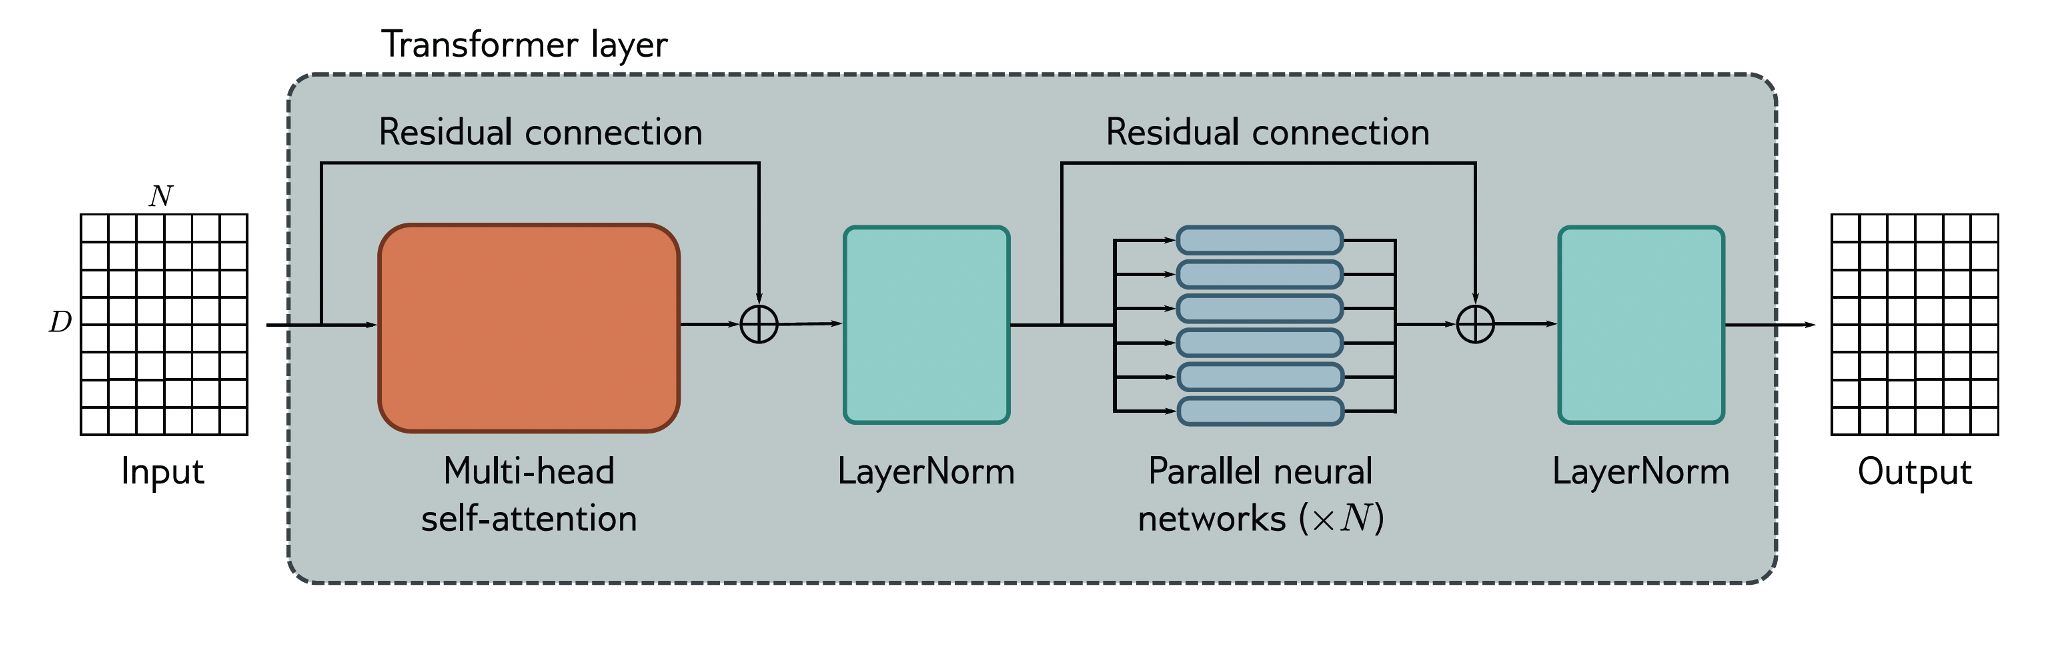
\includegraphics[width=0.9\linewidth]{Section_analysis_tech/Screenshot 2025-08-12 at 14.49.22.png}
    \caption{The transformer takes as input a $D \times N$ matrix, where each of the $N$ columns is the $D$-dimensional embedding of an input object. The output has the same shape. Each transformer layer applies a sequence of operations. First, a multi-headed attention block allows the embeddings to exchange information, producing updated representations for each object. This is done within a residual block, so the original inputs are added back to the attention output. Second, layer normalisation is applied. Third, a second residual block applies the same fully connected feed-forward network independently to each of the $N$ object representations. Finally, layer normalisation is applied again \cite{UDL}.
}
    \label{fig:transformer}
\end{figure}\\
\\
By stacking multiple such layers, the transformer progressively builds rich, context-aware representations that capture both local and global relationships within the event. 
The final representation can then be pooled or otherwise aggregated to produce a compact event-level feature vector, which is passed to a classification head to distinguish $t\bar{t}H(b\bar{b})$ signal events from background processes.
